\documentclass[numbers=noenddot,12pt,a4paper]{scrartcl}
\usepackage[greek,ngerman]{babel}
\usepackage[T1]{fontenc}
\usepackage[utf8]{inputenc}
\usepackage{fullpage}
\usepackage{libertine}
\usepackage{ziffer}
\usepackage{paralist}
\usepackage{graphicx}
\usepackage{units}
\usepackage[infoshow]{tabularx}
\usepackage{amsmath}
\usepackage{amssymb}
\usepackage{wrapfig}
\usepackage{esint}
\usepackage{float}
\usepackage{wrapfig}
\usepackage[font=small]{caption}
\usepackage{subcaption}
\usepackage{lscape}
\usepackage{hyperref}

\renewcommand{\thefigure}{Abb. \arabic{figure}}

\captionsetup[wrapfigure]{name=}
\captionsetup[figure]{name=}
\newcommand{\num}[1]{$\left[\text{#1}\right]$}
\newcommand{\degree}{^\circ}
\newcommand{\diff}{\textnormal{d}}
\newcommand{\tenpo}[1]{\cdot 10^{#1}}
\newcommand{\greek}[1]{\greektext#1\latintext}
\newcommand{\ix}[1]{_\text{#1}}
\newcommand{\imag}{\mathbf{i}}
\newcommand{\tilt}[1]{\textit{#1}}
\newcommand{\grad}[1]{\textit{grad}\left(#1\right)}
\newcommand{\divergenz}[1]{\textit{div}\left(#1\right)}
\newcommand{\euler}{\mathnormal{e}}
\newcommand{\fett}[1]{\textbf{#1}}

\title{Protokoll: Röntgenröhre} %TODO Name des Versuchs eintragen
\author{Philipp Hacker} %TODO Protokollschreiber unterstreichen
\date{\today}

\begin{document}
%\setcounter{page}{2}
%\setcounter{section}{1}
\maketitle
\begin{center}
Betreuer: M. von der Ehe\\ %TODO Name des Betreuers eintragen
Versuchsdatum: 09./10.12.2014\\ %TODO Datum des Versuchs eintragen
\begin{table}[h]
\centering
Note: %TODO Gute Note erhalten :)
\begin{tabularx}{1.5cm}{|X|}
\hline \\ \\
\hline
\end{tabularx}
\end{table}
\end{center}
\vspace*{\fill}
\tableofcontents
\vfill
\newpage
\section{Einleitung}
Die Methode der Röntgenspektroskopie ist Grundlage vieler wichtiger spektroskopischer Untersuchungen wie z.Bsp. Photoelektronenspektroskopie (XPS). Nach seiner Entdeckung 1895 durch \tilt{W. C. Röntgen} wird die Röntgenstrahlung heutzutage nicht nur in der Medizin, sondern auch vermehrt in der Materialphysik und Kristallographie  verwendet. Dabei macht man sich ihre Eigenschaften unter Beugung an Kristallebenen und hohe Strahlungsenergie zur Nutze. Unter anderem ist die chemische Zusammensetzung einer Probe durch die XPS ableitbar, was in der Untersuchung von DNA ausgenutzt wird.\\
In diesem Versuch soll am Beispiel von Eisen, Kupfer und Molybdän die Wechselwirkung von Röntgenstrahlung mit Materie untersucht und nachvollzogen werden. Aus den Ergebnissen dieser Messungen sollen wiederum das \tilt{Duane-Hunt'sche Verschiebungsgesetz} bestätigt und die \tilt{Planck-Konstante} bestimmt werden.
\newpage
\section{Grundlagen}
\subsection{Röntgenstrahlung}
Als Röntgenstrahlung bezeichnet man den Teil des Spektrums elektromagnetischer Strahlung zwischen, je nach Definition$^{\left[\text{I}\right]}$, $\unit[100]{keV}$ und einigen $\unit{MeV}$. In Wellenlängen ,über die $E=hc/\lambda$ Beziehung abgeleitet, ausgedrückt liegt die Röntgenstrahlung zwischen $\unit[10^{-8}]{m}$ und $\unit[10^{-12}]{m}$.\\
Die ionisierende Strahlung kann auf 2 Arten entstehen. Einerseits wird die sie bei der starken Beschleunigung schneller, elektrisch geladener Teilchen in einem  Coulomb-Feld erzeugt. Diese nennt man Bremsstrahlung und ihr Spektrum ist offensichtlich kontinuierlich. Andererseits können Übergänge sehr hoher Energiedifferenzen in der Elektronenhülle Röntgenstrahlung aussenden. Diese Spektrum ist diskret.\\
Die in diesem Versuch genutzte Röntgenröhre nutzt beide Methoden. Die beschleunigt die aus der Glühkathode ausgelösten Elektronen über ein elektrisches Feld, wobei sie die kinetische Energie $E\ix{kin}=qU\ix{B}=eU\ix{B}$ erhalten. Dabei ist $U\ix{B}$ die Potentialdifferenz zwischen Kathode und Anode. Die hochenergetischen Elektronen treffen auf die Anode und können dort mehrere Effekte auslösen. Zum einen kann eine eintreffendes Elektron im Coulomb-Feld der Atome abgebremst und in seiner Flugbahn abgelenkt werden. Dadurch entsteht die Bremsstrahlung. Weiterhin ist es möglich, dass eines der schnellen Elektronen durch den Stoß mit einem Teilchen in der Hülle eines Anoden-Atoms eine Niveau-Änderung stimuliert. Die Relaxation dieses Zustandes sendet die für das Anodenmaterial charakteristische Röntgestrahlung aus.\\
Es sei erwähnt, das die Photonen beider Abstrahlprozesse noch mit dem Anodenmaterial wechselwirken können. Anwendung findet dieser Effekt in der Röntgenphotoelektronenspektroskopie \tilt{XPS}$^{\left[\text{II}\right]}$. Dabei werden Elektronen unterer Schalen angeregt und in höhere Zustände gehoben. Wo genau das Elektron sich einsetzt und damit die Eigenschaften des Atoms verändert, hängt von dessen Ausgangszustand und der Anregung ab. Nach der Anhebung des Niveaus löst sich das Elektron aus der Elektronenhülle, wobei die verbleibende kinetische Energie über den Ausgangszustand vor der Anregung bestimmt ist.
\newpage
\subsection{Bragg-Reflexion}
Trifft Röntgenstrahlung auf einen Kristall, so durchdringt diese fast vollständig den Festkörper. Ein Teil jedoch wird an seiner Gitterstruktur gebeugt. Die Röntgenbeugung findet an den verschiedenen Ebenen des Kristalls statt, für die gerade die sogenannten \tilt{Bragg-Bedingung} erfüllen$^{\left[\text{III}\right]}$ (siehe Gl. \ref{eq:bragg}).\\
Die einlaufenden Wellen stehen mit ihrem Wellenvektor im Winkel $\alpha$ zum Lot und haben damit den Bragg-Winkel $\theta=90\degree-\alpha$ (siehe \ref{img:bragg}). Bei koheränter Strahlung muss der Gangunterschied $\delta$ zwischen einer an den oberen und unteren Gitterebenen reflektierten Welle ein vielfaches der Wellenlänge $\lambda$ sein. Außerdem lässt sich über eine Winkelbeziehung $\delta=d\sin\left(\theta\right)$ finden. Zusammenführen ergibt die besagte \tilt{Bragg-Bedingung}.
\begin{align}
	n\lambda=2d\sin\left(\theta\right) \label{eq:bragg}
\end{align}
\begin{figure}[H]
	\centering
	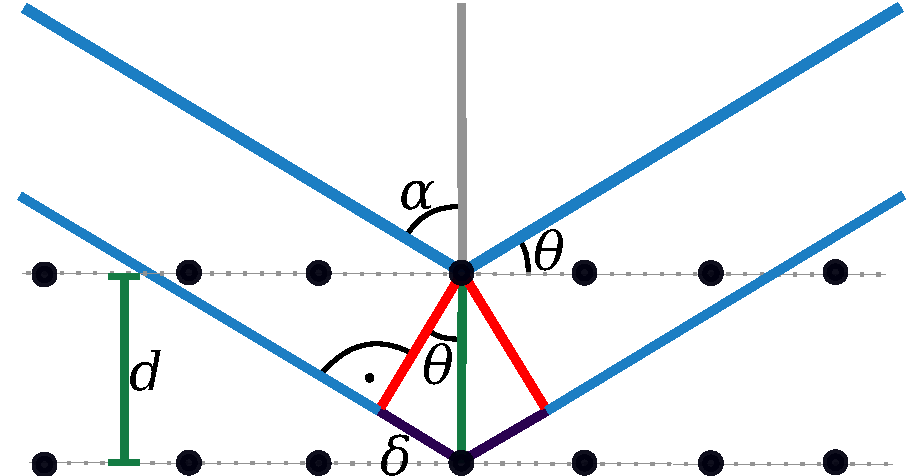
\includegraphics[width=0.5\textwidth]{bragg.pdf}
	\caption{$2$\,-\,$\theta$\,-\,Anordnung an Kristallebenen mit dem Abstand $d$ und einfallenden Wellen}\label{img:bragg}
\end{figure}
\subsection{Duane-Hunt-Verschiebung}
Wie bereits beschrieben erfahren die aus der Glühkathode der Röntgenröhre ausgelösten Elektronen an der Anode eine negative Beschleunigung. Dabei kann ihre gesamte kinetische Energie in Strahlungsenergie übergehen. Mit dieser maximalen Bremsstrahlung korreliert eine minimale Wellenlänge $\lambda\ix{min}$. \tilt{W. Duane} und \tilt{F. Hunt} konnten 1915 den in Gl. (\ref{eq:verschieb}) gezeigten Zusammenhang empirisch beweisen. Nimmt man weiterhin die Beziehungen über die kinetische Energie der Elektronen und die Energie der Röntgenphotonen hinzu, so folgt Gl. (\ref{eq:lambda}). Die Übereinstimmung bestätigt somit das Experiment und die gemachten Annahmen.
\begin{align}
	U\ix{B}\cdot\lambda\ix{min}\propto\unit[1,25\cdot 10^{-6}]{Vm} \label{eq:verschieb} \\
	\lambda\ix{min}=\frac{h\cdot c}{e\cdot U\ix{B}}=\frac{\unit[1,2398\cdot 10^{-6}]{Vm}}{U\ix{B}} \label{eq:lambda}
\end{align}
\newpage
\subsection{Röntgenspektroskopie}
Im folgenden soll die Röntgenspektroskopie am Beispiel dieses Versuches erläutert werden.\\
Legt man in die, in \ref{img:bragg} gezeigte $2$\,-$\theta$\,-\,Anordnung, hinter den Lithiumfluorid-Kristall einen Detektor, so lässt sich, nach Gl. (\ref{eq:bragg}), die erzeugte Röntgenstrahlung als ein Energiespektrum vermessen. Mit der minimalen Wellenlänge $\lambda\ix{min}$ korrespondiert dabei ein minimaler Bragg-Winkel $\theta\ix{min}$. Im Detektor erfahren gerade die Strahlen, welche der Bragg-Bedingung Gl. (\ref{eq:bragg}) genügen, eine konstruktive Interferenz. Dabei wird ein Zählrohr verwendet, welches die Intensität in Form von Photonen-Impulsen pro Sekunde $\unit{Imp/s}$ misst. Ein geeigneter Aufbau (siehe \ref{img:aufbau}) lässt die entsprechende Winkelveränderung bezüglich des Röntgenstrahls bei fester Quelle zu. Eine solche Konstruktion nennt man Goniometer. Für diesen Aufbau erwartet man ein Spektrum wie in \ref{img:spektr} mit den charakteristischen Peaks und dem Anteil der Bremsstrahlung bis $\lambda\ix{min}$. Dabei verläuft die Skala analog: kleine Winkel bedeuten kleine Wellenlängen und damit große Energien.\\
Die Spannung zwischen Kathode und Anode $U\ix{B}$ kann  in diesem Versuch bis $\unit[35]{kV}$ geregelt werden. Dies entspricht einer kinetischen Energie von $\unit[40]{keV}$ und damit einer Wellenlänge von $\unit[35]{pm}$. Der Strom durch den Glühdraht ist relativ gering und beträgt $\unit[1]{mA}$. Es ist möglich, die Messung für einen Winkel über ein bestimmtes Zeitintervall durchzuführen und damit die Intensität schließlich darüber zu mitteln.\\
Unter Erhöhung der Spannung $U\ix{B}$ verschiebt sich $\lambda\ix{min}$ zu geringeren Werten und beschreibt damit größere Energien. Die Position der charakteristischen Peaks verändert sich dabei nicht, wobei jedoch die Intensität insgesamt erhöht wird.
\begin{figure}[H]
	\centering
	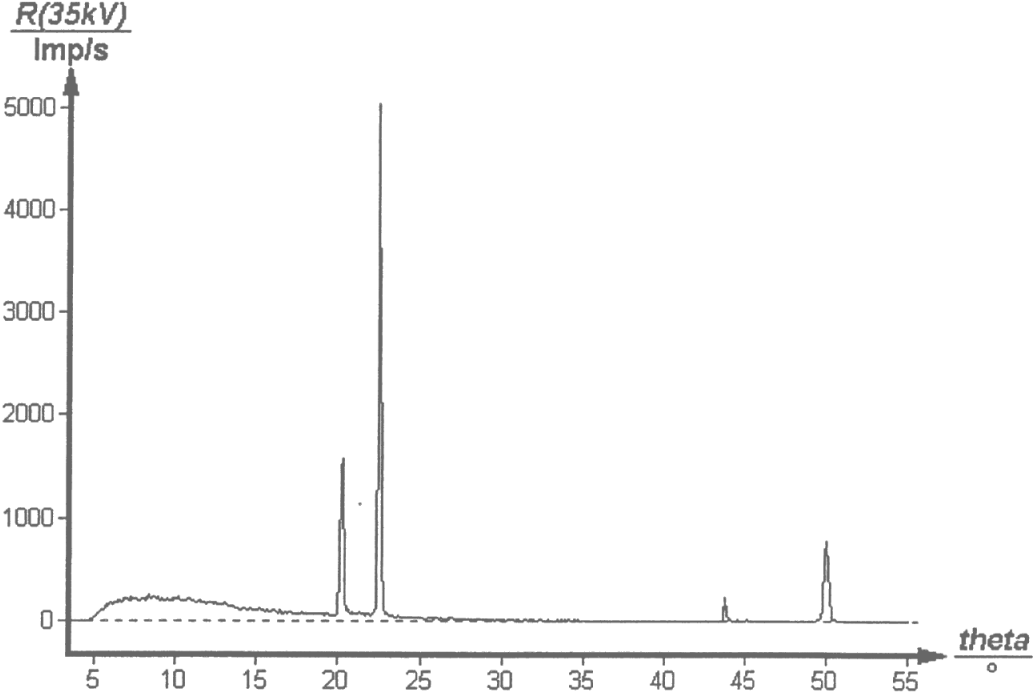
\includegraphics[width=0.7\textwidth]{spektrum.png}
	\caption{Beispielspektrum einer Kupferanode, LiF-Kristall im Goniometer}\label{img:spektr}
\end{figure}
\newpage
\section{Durchführung}
Für die Anodenmaterialien Kupfer, Molybdän und Eisen werden die Röntgenspektren aufgenommen. Eingangs wird jeweils ein 'Referenzspektrum' bei $\unit[33]{kV}$ zwischen $3,5\degree$ und $55\degree$ bzw. $60\degree$ mit Schritten von $0,1\degree$ aufgenommen. Das Zeitintervall, die sogenannten Integrationszeit, beträgt hierbei $\unit[2]{s}$.\\
Anschließend wird für jedes Anodenmaterial ein detaillierteres Spektrum entsprechend der Lage ihrer charakteristischen Peaks aufgenommen. Dabei wird die Beschleunigungsspannung zwischen $\unit[15]{kV}$ und $\unit[31]{kV}$ mit $\unit[2]{kV}$-Schritten verändert. Dafür wurde die Integrationszeit konstant gelassen und der Winkelbereich eingeschränkt. Die verwendetet Röntgenröhre mit Anschluss an einen PC, Goniometer und LiF-Kristall-Anordnung zeigt \ref{img:aufbau}.
\begin{figure}[H]
	\centering
	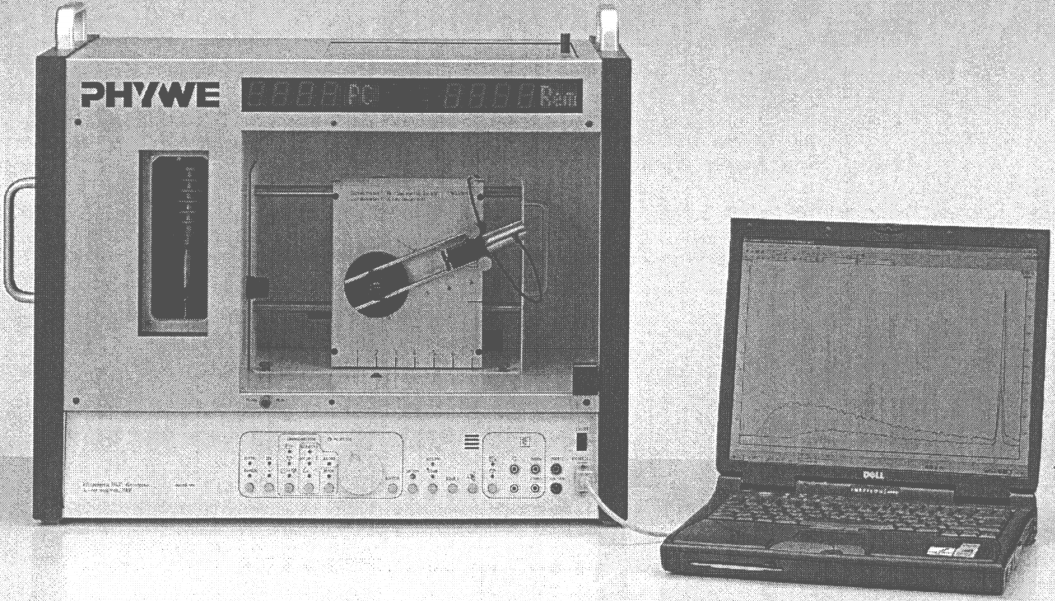
\includegraphics[width=\textwidth]{aufbau.png}
	\caption{Röntgenröhre mit Goniometer und $2$\,-\,$\theta$\,-Anordnung} \label{img:aufbau}
\end{figure}
\newpage
\section{Auswertung}
\subsection{Charakteristischen Linien}
In Abbildung \ref{tab:charak} sind die Spektren aller 3 Anodenmaterialien zusammen dargestellt. Klar heraus stechen dabei die charakteristischen Peaks eines jeden Materials, die abhängig von der inneren Struktur sind. In der sich anschließenden Tabelle \ref{tab:charak} sind die jeweiligen Wellenlängen und korrespondierenden Energien für diese angegeben. Dabei unterscheiden sich die Messergebnisse nur um eine $\unit{pm}$ von den gegebenen Literaturwerten (siehe \num{V}). Der Unterschied zwischen charakteristischem und kontinuierlichem Bremsspektrum wurde hierbei sehr deutlich. Die besagten Intensitätsmaxima sind außerdem unabhängig von der Anodenspannung (siehe \ref{subsec:mess}), was diese Erkenntnis bekräftigt.
\begin{figure}[H]
	\centering
	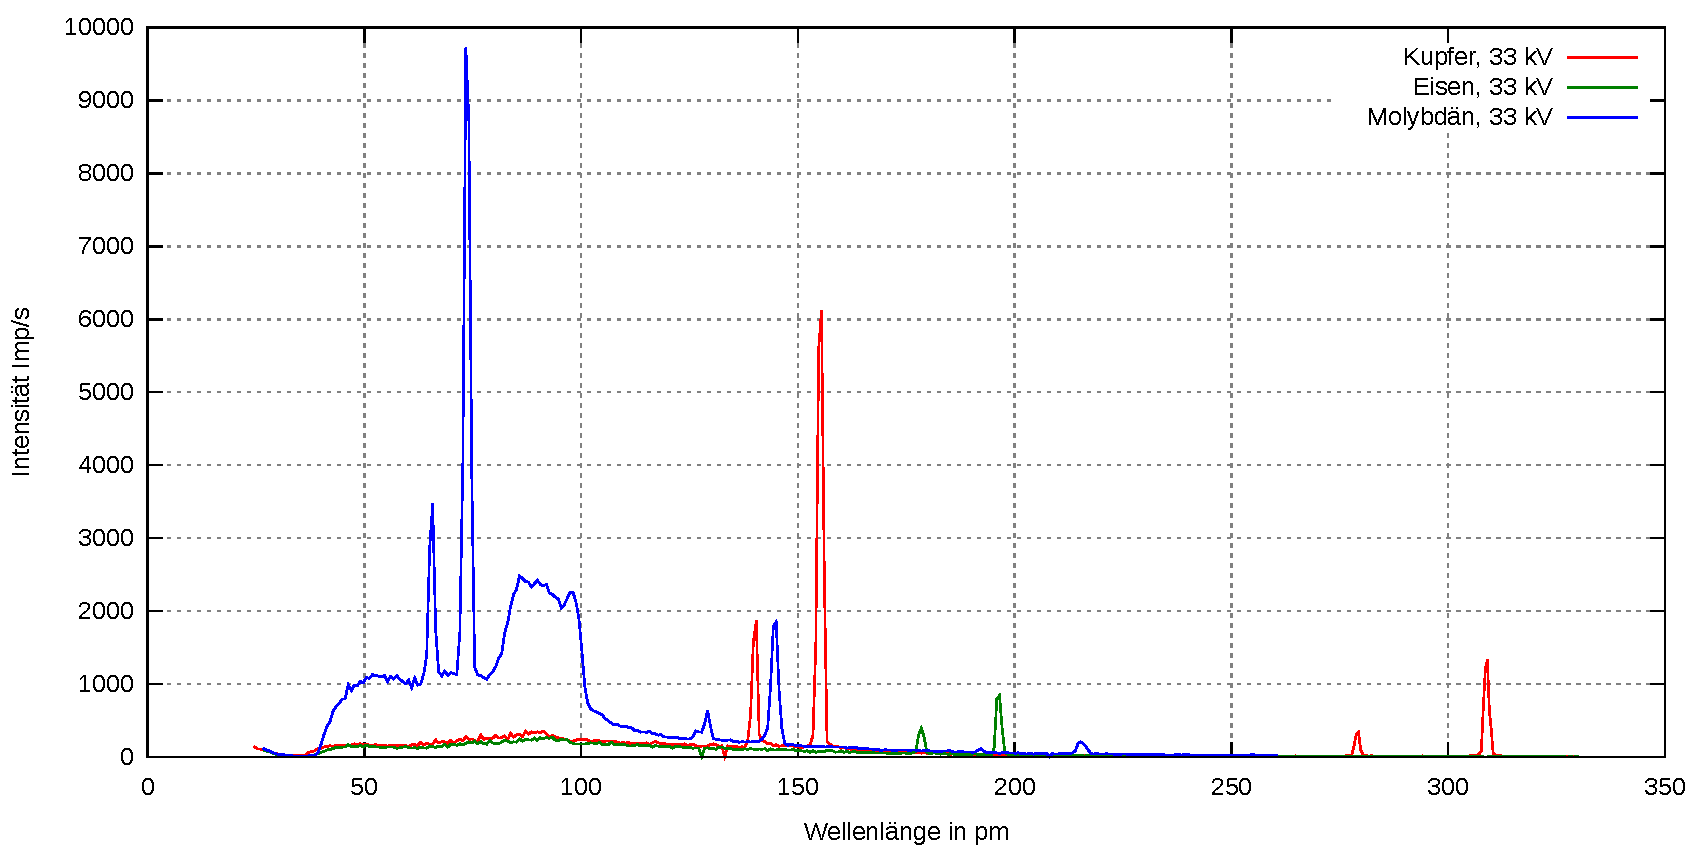
\includegraphics[width=\textwidth]{spektren.pdf}
	\caption{Referenzspektren der versch. Materialien bei $\unit[33]{kV}$ und $\unit[1]{mA}$}\label{img:refere}
\end{figure}
\begin{table}[H]
	\centering
	\begin{tabular}{c|c|c|c|c}
		Anodenelement & $\lambda_\alpha$/pm & $E_{K_{\alpha}}$/eV & $\lambda_{\beta}$/pm & $E_{K_{\beta}}$/eV \\ \hline
		Kupfer & $155,449$ & $7975,9$ & $140,409$ & $8830,5$ \\ \hline
		Eisen & $196,24$ & $6381$ & $178,458$ & $6947,5$ \\ \hline
		Molybdän & $73,54$ & $16859$ & $65,61$ & $18897$ \\ \hline
	\end{tabular}
	\caption{Wellenlängen $\lambda$ der charakteristischen Linien im Spektrum der Anodenmaterialien}\label{tab:charak}
\end{table}
\subsection{Duane-Hunt-Gesetz und Planck-Konstante}
Im Anschluss sind Detailaufnahmen der Spektren einer jeden Anode für die Beschleunigungsspannungen $\unit[15-31]{kV}$ gezeigt. Hieraus lassen sich leicht die in \ref{tab:min} aufgeführten Abschneidewellenlängen $\lambda\ix{min}$ ablesen. Etwaiges Rauschen bzw. verbleibende Restintensität, oder sogar ein erneutes Ansteigen der Impulszahlen, kann durch die offene Konstruktion des Goniometers und der $2$\,-\,$\theta$\,-\,Anordnung erklärt werden: der Kristall (u.U. auch Blende) beugt nicht nur die Strahlung, sondern streut sie auch in den gesamten Aufbau.\\
Offensichtlich verschiebt sich die minimale Wellenlänge zu größeren Energien für höhere Anodenspannungen, was ebenso einsichtig ist, da ja diese gleichbedeutend sind mit größeren kinetischen Energien der Elektronen.
\begin{figure}[H]
	\centering
	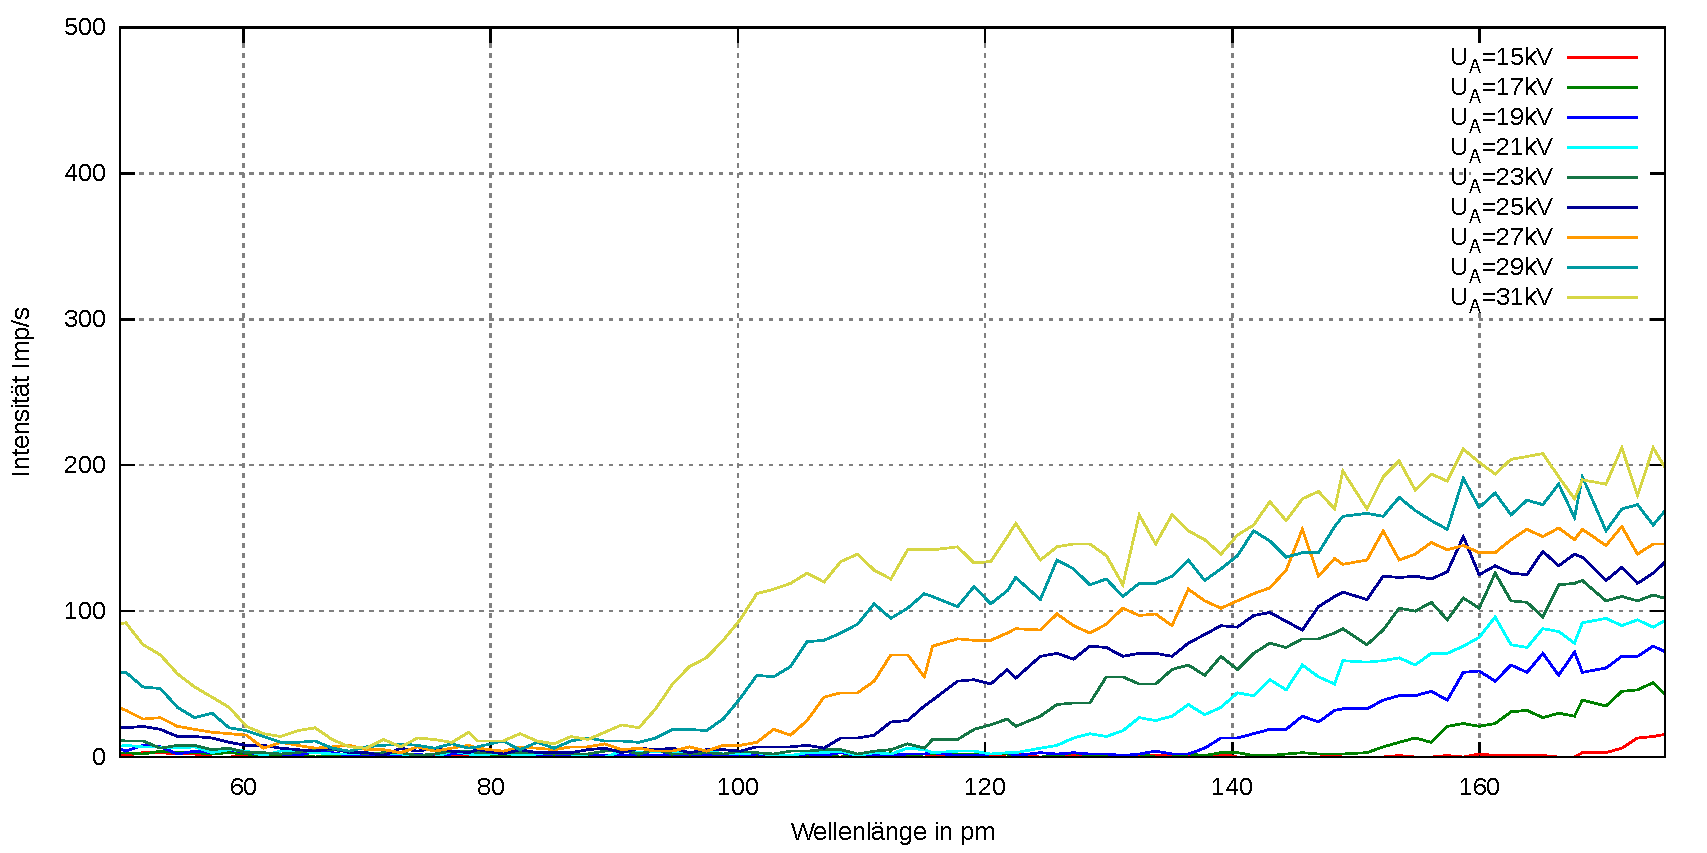
\includegraphics[width=\textwidth]{kupfermin.pdf}
	\caption{Nahaufnahme der niedrigsten Wellenlängen von Kupfer über versch. Spannungen} \label{img:cumin}
\end{figure}
\begin{figure}[H]
	\centering
	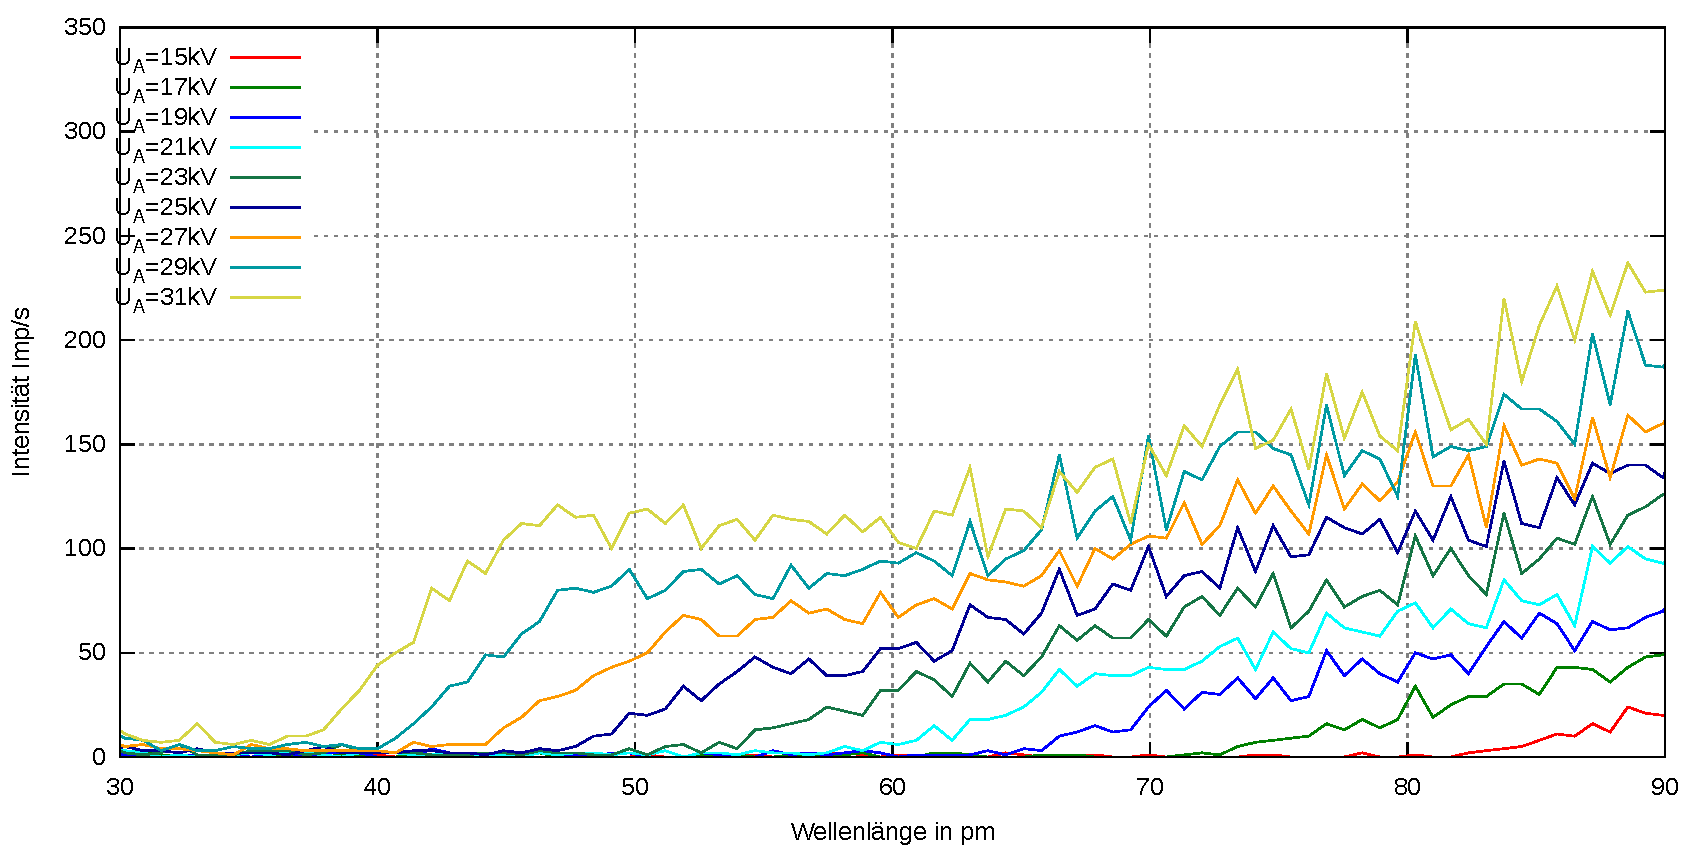
\includegraphics[width=\textwidth]{eisenmin.pdf}
	\caption{Nahaufnahme der niedrigsten Wellenlängen von Eisen über versch. Spannungen} \label{img:femin}
\end{figure}
	
\begin{figure}[H]
	\centering
	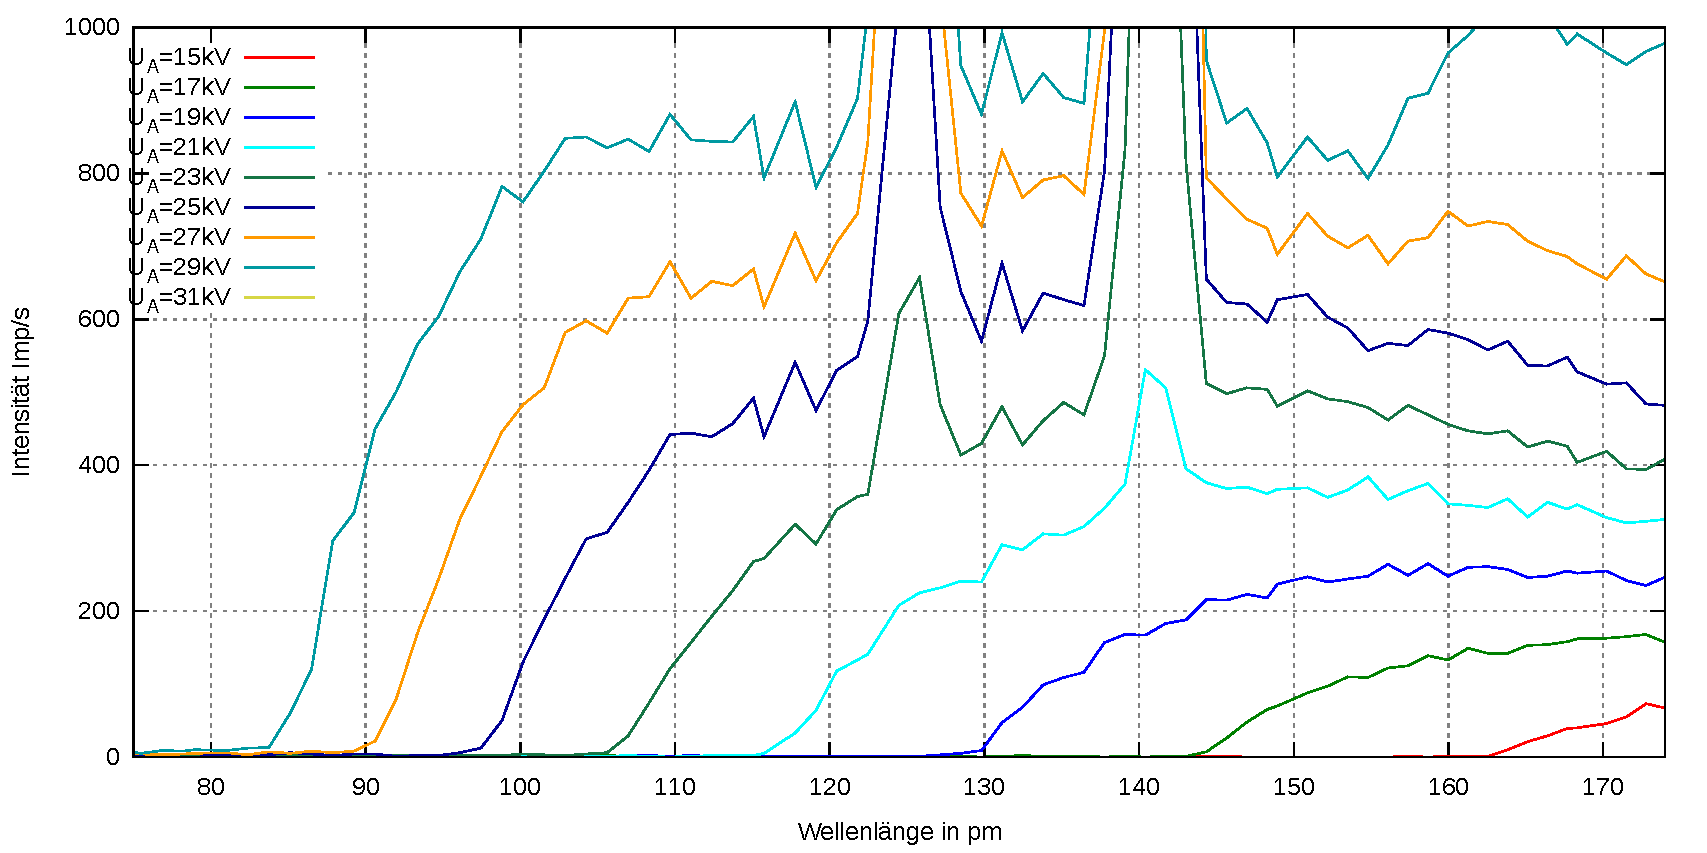
\includegraphics[width=\textwidth]{molymin.pdf}
	\caption{Nahaufnahme der niedrigsten Wellenlängen von Molybdän über versch. Spannungen} \label{img:momin}
\end{figure}

\begin{table}[H]
	\centering
	\begin{tabular}{c|c|c|c}
		Wellenlängen &  Kupfer & Eisen & Molybdän \\ \hline
		$\lambda\ix{min}(\unit[15]{kV})$/pm & $168,02$ & $81,7$ & $\textsc{162,6}$\\ \hline
		$\lambda\ix{min}(\unit[17]{kV})$/pm & $150,41$ & $72,6$ & $144,31$ \\ \hline
		$\lambda\ix{min}(\unit[19]{kV})$/pm & $136,53$ & $64,95$ & $129,73$ \\ \hline
		$\lambda\ix{min}(\unit[21]{kV})$/pm & $122,4$ & $58,4$ & $115,7$ \\ \hline
		$\lambda\ix{min}(\unit[23]{kV})$/pm & $114,7$ & $52,5$ & $105,6$ \\ \hline
		$\lambda\ix{min}(\unit[25]{kV})$/pm & $107,04$ & $46,7$ & $97,2$\\ \hline
		$\lambda\ix{min}(\unit[27]{kV})$/pm & $101,52$ & $43,42$ & $89,5$\\ \hline
		$\lambda\ix{min}(\unit[29]{kV})$/pm & $94,6$ & $39,9$ & $83,6$ \\ \hline
		$\lambda\ix{min}(\unit[31]{kV})$/pm & $88,9$ & $36,34$ & NaN\\ \hline
	\end{tabular}
	\caption{Minimale Wellenlängen der versch. Materialien bei entsprechenden Spannungen}\label{tab:min}
\end{table}
Schließlich kann man aus den Werten in \ref{tab:min} das in Gl. (\ref{eq:verschieb}) besprochene Veschiebungsgesetz nach Duane und Hunt verifizieren. Hierfür macht man einen einfachen Ansatz einer Gerade ohne Offset in der Vertikalen $f(1/U\ix{B})=f(x)=m\cdot x$. Diese Annahme benutzt man nun für einen Fit über die Messdaten einer Anode und sieht damit in \ref{img:duane}, dass das Produkt aus Spannung und Abschneidewellenlänge konstant ist. \\
Hierbei kann man den Anstieg wiederum zur Bestimmung der Fundamentalkonstante $h$, dem \tilt{Planckschen Wirkungsquantum} benutzen. Der Anstieg ist nämlich gerade $m=h\cdot c/e$. Die ermittelten Werte zeigen Gl. (\ref{eq:h1})-(\ref{eq:h2}). Der Fakt, dass mehrere Ergebnisse erzielt wurden, zeugt nicht von der großen Genauigkeit der Methode zur Bestimmung dieser Konstante. Andererseits ist es möglich, dass für die jeweiligen Anoden eine grundlegender Experimentierfehler vorlag und deswegen die Messung an Aussagekraft verlor. Jedoch ist es befriedigend, dass unser Wert für Eisen sehr nahe am wahren Wert liegt.
\begin{figure}[H]
	\centering
	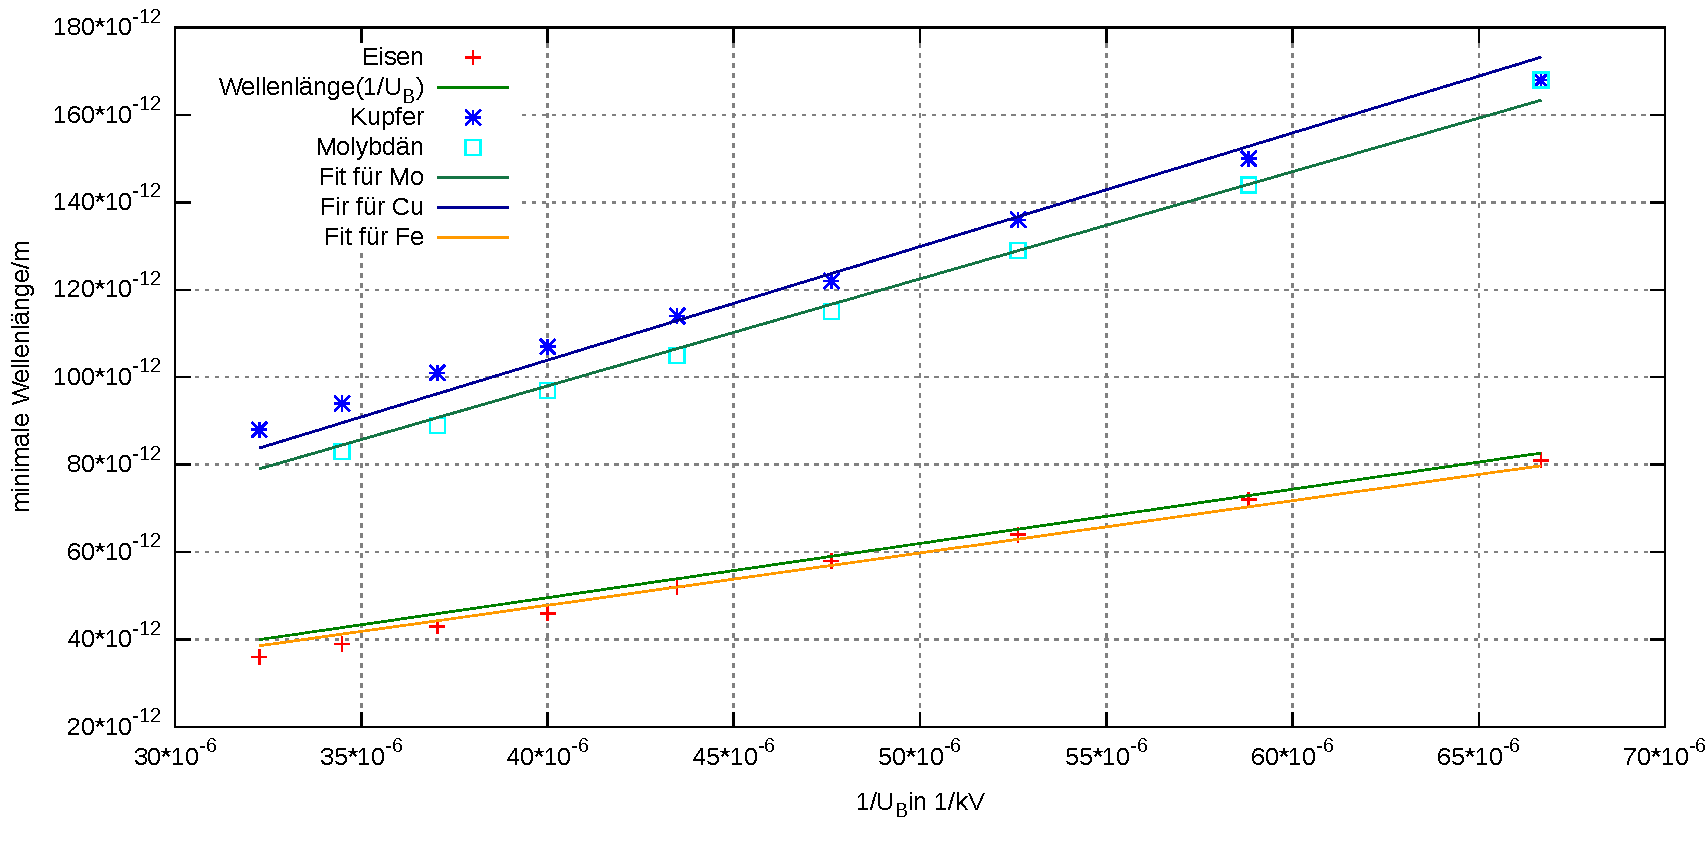
\includegraphics[width=\textwidth]{duane.pdf}
	\caption{Duane-Hunt-Gesetz im Vergleich zu den Messpunkten und deren Fit}\label{img:duane}
\end{figure}
\begin{align}
	h\ix{Cu}=\unit[1,38844\cdot10^{-33}]{Js} \label{eq:h1}\\
		h\ix{Fe}=\unit[6,3929\cdot10^{-34}]{Js} \\
			h\ix{Mo}=\unit[1,30951\cdot10^{-33}]{Js} \label{eq:h2}
\end{align}
\subsection{Messwerte}\label{subsec:mess}
\begin{figure}[H]
	\centering
	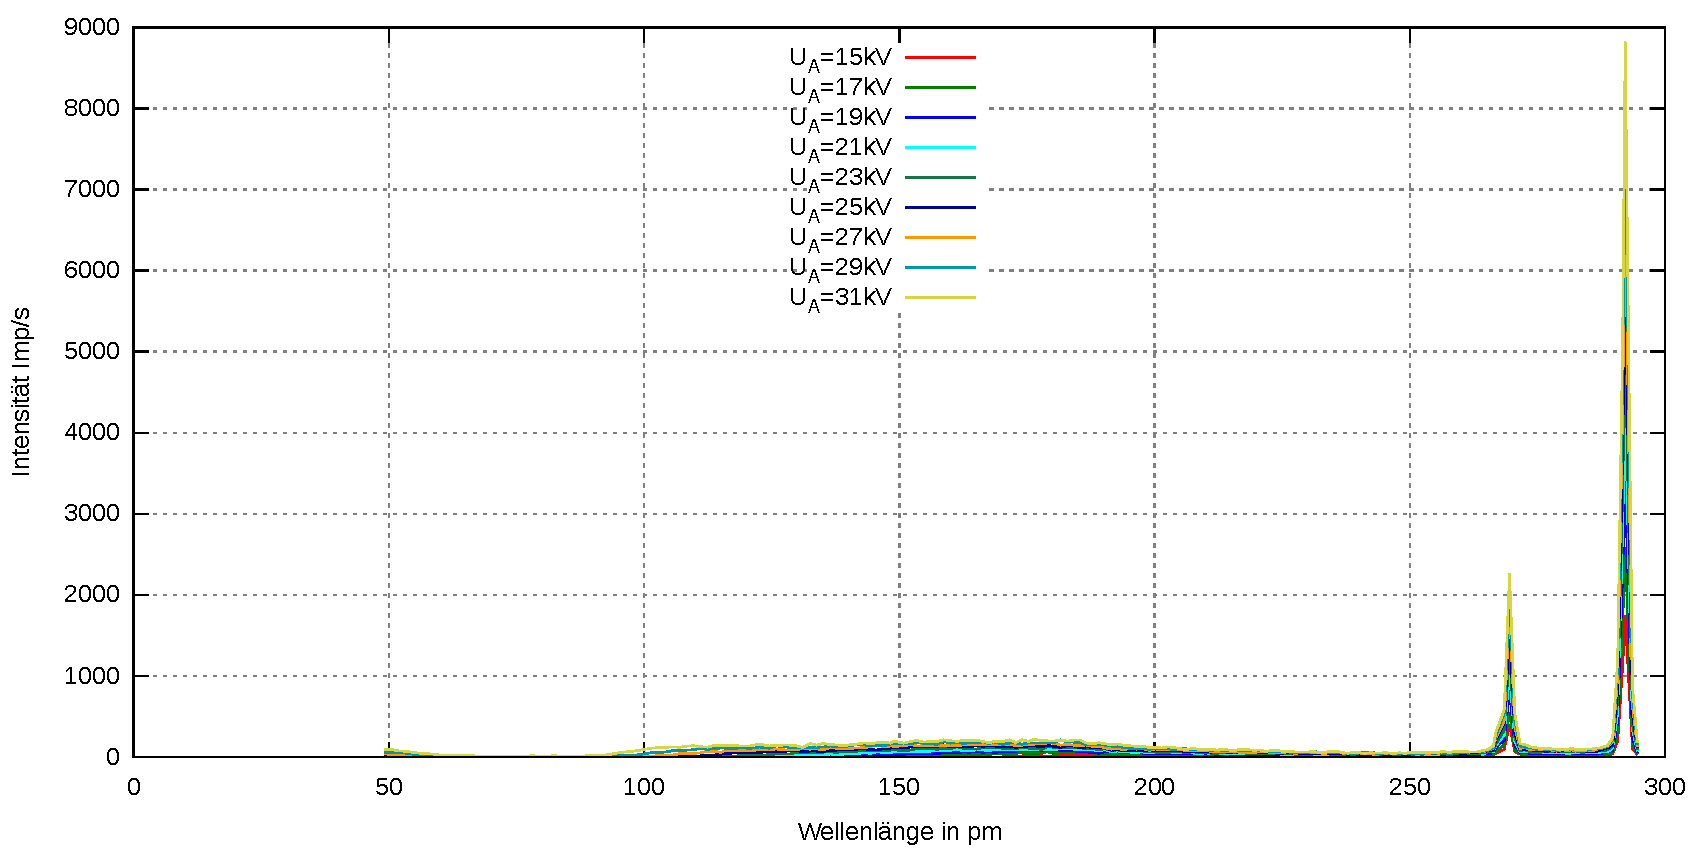
\includegraphics[width=\textwidth]{kupferges.pdf}
	\caption{Röntgenspektrum einer Kupferanode ($\unit[15-31]{kV}$ Anodenspannung, $\unit[1]{mA}$ Anodenstrom)}
\end{figure}

\begin{figure}[H]
	\centering
	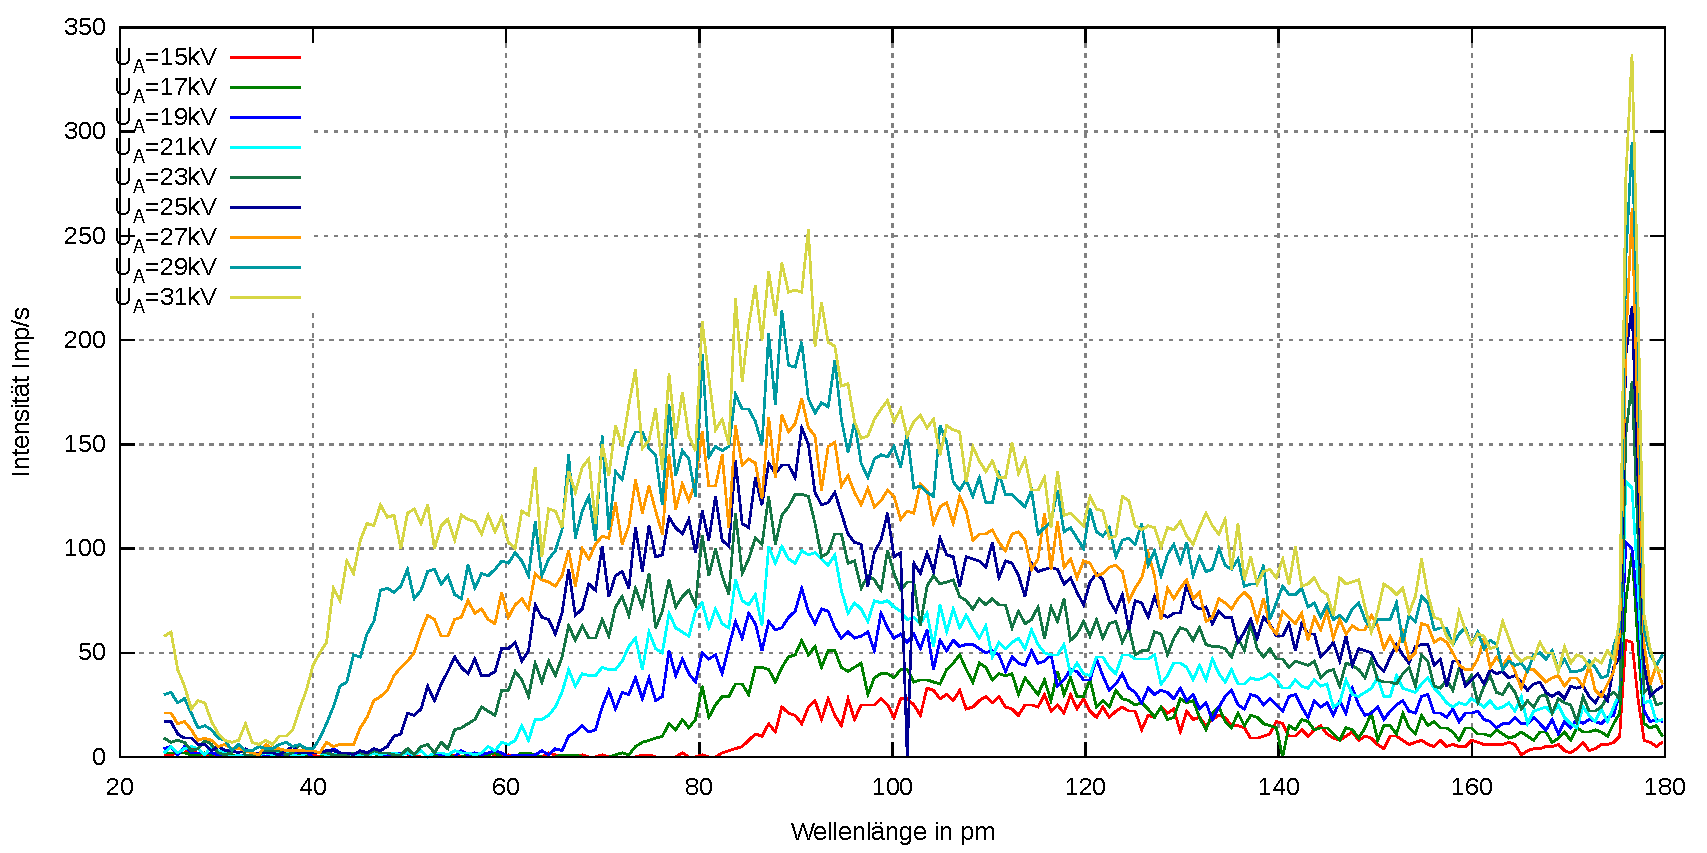
\includegraphics[width=\textwidth]{eisenges.pdf}
	\caption{Röntgenspektrum einer Eisenanode ($\unit[15-31]{kV}$ Anodenspannung, $\unit[1]{mA}$ Anodenstrom)}
\end{figure}

\begin{figure}[H]
	\centering
	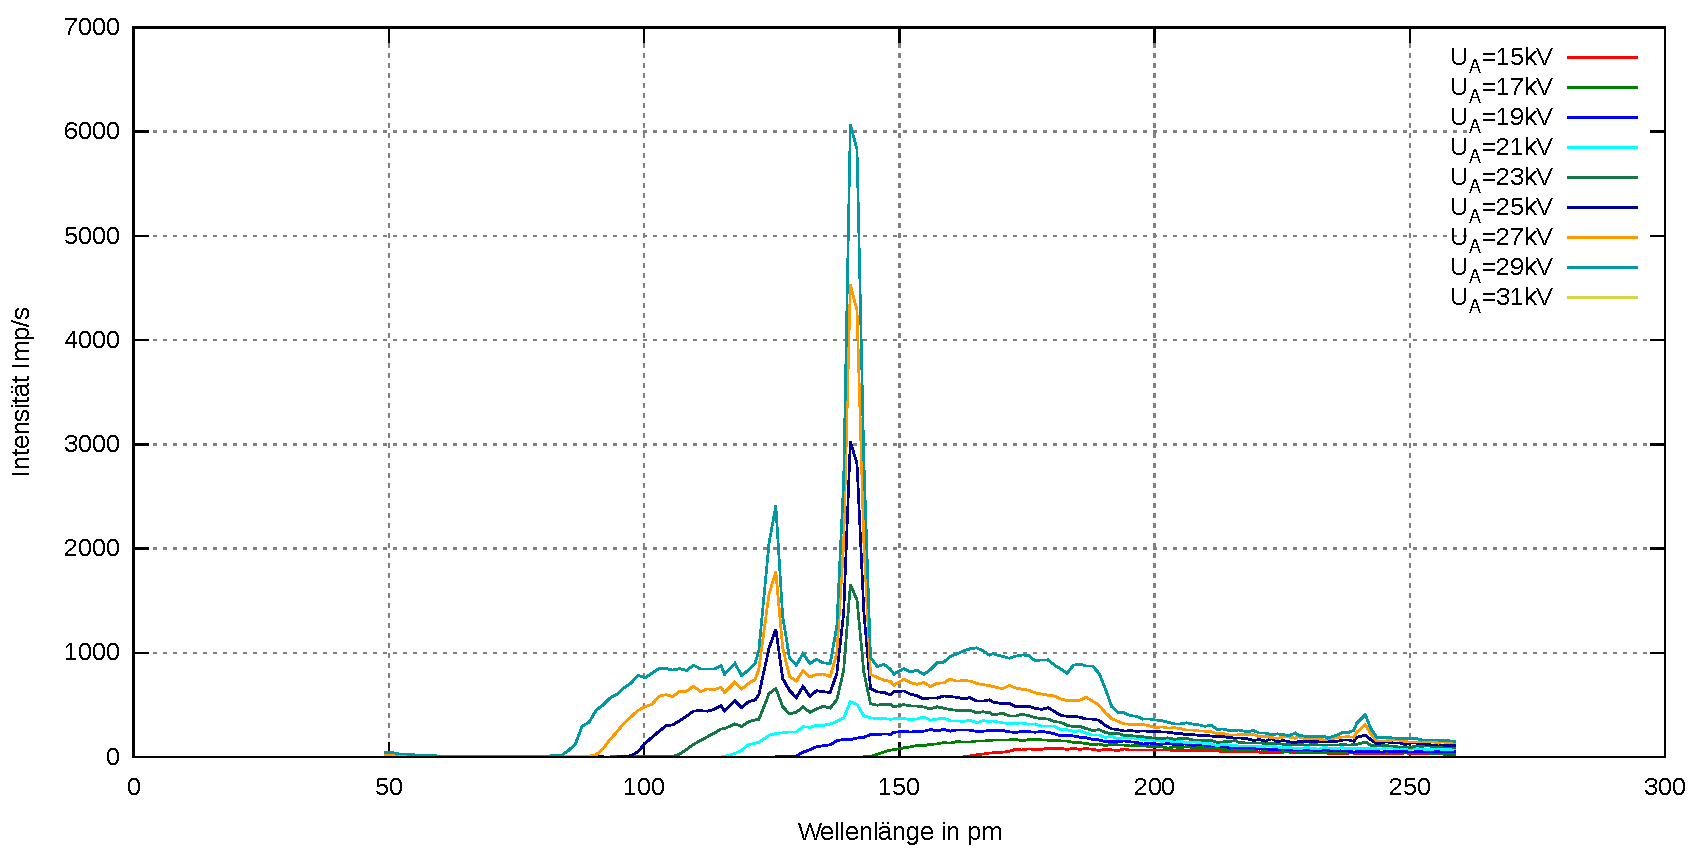
\includegraphics[width=\textwidth]{molyges.pdf}
	\caption{Röntgenspektrum einer Molybdänanode ($\unit[15-31]{kV}$ Anodenspannung, $\unit[1]{mA}$ Anodenstrom)}
\end{figure}
\newpage
\section{Quellen}
	\num{I} -- \url{http://de.wikipedia.org/wiki/R%C3%B6ntgenstrahlung}\\ \\
	\num{II} -- \dots\url{/wiki/R%C3%B6ntgenphotoelektronenspektroskopie}\\ \\
	\num{III} -- \dots\url{/wiki/Bragg-Gleichung}\\ \\
	\num{IV} -- \dots\url{/wiki/Bragg-Gleichung}; Abschn.: "`Herleitung"', Abb. 1 \\ \\
	\num{V} -- Versuchsanleitung "`Röntgenröhre"'; Abschn.: Auswertung u. Durchführung, Abb. 2
\end{document}